\documentclass[10pt,landscape]{article}
\usepackage{multicol}
\usepackage{calc}
\usepackage{ifthen}
\usepackage[landscape]{geometry}
\usepackage{listings}
\usepackage{amsmath,amsthm,amsfonts,amssymb}
\usepackage{mathtools}
\usepackage{color,graphicx,overpic}
\usepackage{hyperref}
\usepackage[dvipsnames]{xcolor}

\usepackage{MnSymbol}
\usepackage{graphicx}
\usepackage{wrapfig}

\usepackage{blindtext}

% This sets page margins to .1 inch if using letter paper, and to 1cm
% if using A4 paper. (This probably isn't strictly necessary.)
% If using another size paper, use default 1cm margins.
\ifthenelse{\lengthtest { \paperwidth = 11in}}
    { \geometry{top=0.2in,left=0.2in,right=0.2in,bottom=0.2in} }
    {\ifthenelse{ \lengthtest{ \paperwidth = 297mm}}
        {\geometry{top=1cm,left=1cm,right=1cm,bottom=1cm} }
        {\geometry{top=1cm,left=1cm,right=1cm,bottom=1cm} }
    }

% Turn off header and footer
\pagestyle{empty}

% Redefine section commands to use less space
\makeatletter
\renewcommand{\section}{\@startsection{section}{1}{0mm}%
                                {-1ex plus -.5ex minus -.2ex}%
                                {0.5ex plus .2ex}%x
                                {\normalfont\large\bfseries}}
\renewcommand{\subsection}{\@startsection{subsection}{2}{0mm}%
                                {-1ex plus -.5ex minus -.2ex}%
                                {0.5ex plus .2ex}%
                                {\normalfont\normalsize\bfseries}}
\renewcommand{\subsubsection}{\@startsection{subsubsection}{3}{0mm}%
                                {-1ex plus -.5ex minus -.2ex}%
                                {0.5ex plus .2ex}%
                                {\normalfont\small\bfseries}}
\makeatother

% Itemize to use less space
\usepackage{enumitem}
\setlist{leftmargin=*, nosep}
\setenumerate{nosep}

% Define BibTeX command
\def\BibTeX{{\rm B\kern-.05em{\sc i\kern-.025em b}\kern-.08em
    T\kern-.1667em\lower.7ex\hbox{E}\kern-.125emX}}

% Don't print section numbers
\setcounter{secnumdepth}{0}


\setlength{\parindent}{0pt}
\setlength{\parskip}{0pt plus 0.5ex}

%My Environments
\newtheorem{example}[section]{Example}

\newcommand{\Blue}[1]{\noindent{\textbf{\textcolor{Blue}{#1 -}}}}
\newcommand{\Red}[1]{\noindent{\textbf{\textcolor{BrickRed}{#1 -}}}}
\newcommand{\Green}[1]{\noindent{\textbf{\textcolor{PineGreen}{#1 -}}}}
\newcommand{\Hint}[1]{\noindent{\textcolor{Orange}{#1}}}
% -----------------------------------------------------------------------

\begin{document}
\raggedright
\footnotesize

\begin{multicols}{4}
% multicol parameters
% These lengths are set only within the two main columns
%\setlength{\columnseprule}{0.25pt}
\setlength{\premulticols}{1pt}
\setlength{\postmulticols}{1pt}
\setlength{\multicolsep}{1pt}
\setlength{\columnsep}{2pt}

\subsection{Consumer Demand}

\Blue{Willingness To Pay (WTP)} The most a consumer will pay for a good.

\Red{Consumer Demand} For each price $P$ what quantity is demanded? $Q = Q_D (P)$. \textbf{Inverse demand}: the price at which quantity Q could be sold. $P = P_D (Q)$

\begin{wrapfigure}{r}{0.75\columnwidth}
    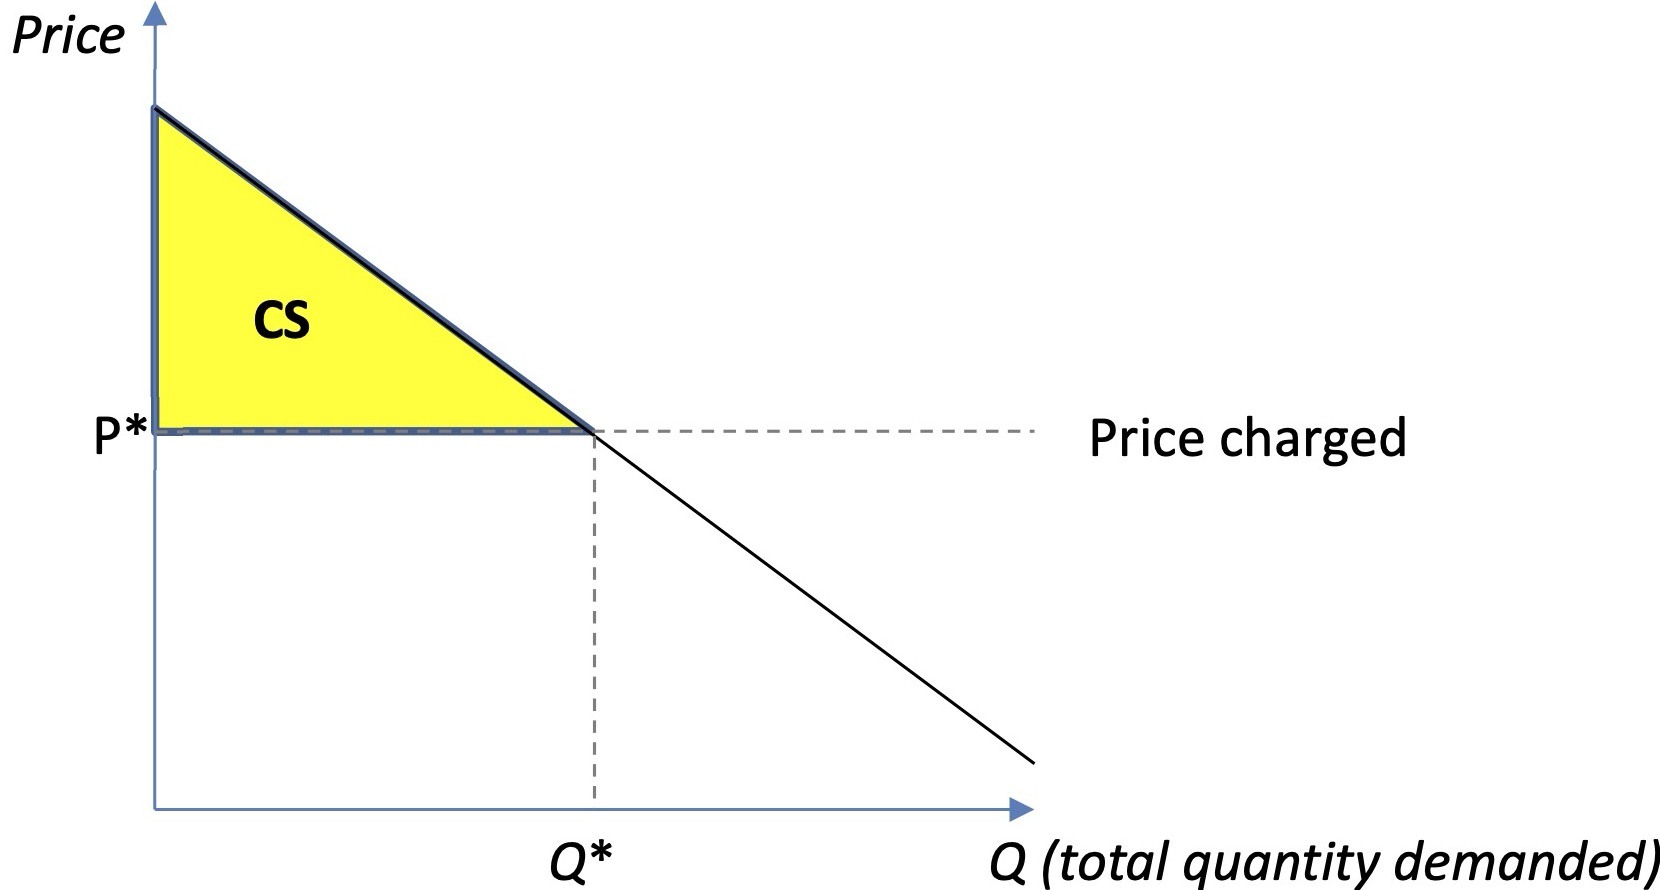
\includegraphics[width=0.75\columnwidth]{CS.jpg}
\end{wrapfigure}
\Red{Consumer Surpluse} Area below demand curve and above price paid.

\Blue{Elasticity} meansure of price sensitivity
\Green{Own-price elasticity of demand $\frac{\% \Delta Q_1^D}{\% \Delta P_1}$} the \% change in quantity demanded for a
1\% change in its price. Always negative by Law of Demand. $|E| \begin{cases}
    < 1 & \text{Inelastic} \\
    > 1 & \text{Elastic}
\end{cases}$

\Green{Cross-price elasticity of demand $\frac{\% \Delta Q_1^D}{\% \Delta P_2}$} the \% change in quantity demanded for a
1\% change in \underline{another good's} price. $\begin{cases}
    > 0 & \text{SUBSTITUTES (wine \& beer)} \\
    < 0 & \text{COMPLEMENTS (popcorn \& beer)}
\end{cases}$

\subsection{Demand Estimation}

\Red{Demand Shifts} Any change in the envrionment that changes demand other than price. E.g. before and after advertising.

\Blue{Estimation Techniques}
\begin{enumerate}
    \item Randomized Control Trials: A/B tests. Considered the \underline{gold standard} for demand estimation because
        of their ability to establish causality. In a randomized experiment, subjects are randomly allocated to
        different prices and this allows us to attribute the change in demand to price changes rather than to some other
        confounding variable.
    \item ``Nautral'' or ``Quasi-'' experiments: when price variation is ``as good as random'' (e.g. demand just above
        or below price-surge threshold).
\end{enumerate}

\Green{Equity Tradeoffs} different equity objectives may exist in different applications. Continuous algorithmic
testing, penalties for disparities, affirmative information potential solutions.

\subsection{Costs}

\Blue{Sunk Cost} costs that are unavoidable and cannot be recovered. Whether a cost is sunk or not depends on the timing
of the business decision.

\Blue{Opportunity Cost} the highest valued alternative use of an input; an example is ``no such thing as a free lunch'':
you could do something else with your time. Example of Capital: Rate of return on the next best alternative use of funds
(relative to the current business decision).

\Blue{Fixed Cost} costs that don't vary with the level of output (Q).

\Blue{Variable Cost} costs that vary with the level of output (Q).

The fixed vs variable cost distinction depends on the business question and on the time horizon. E.g., all inputs
(including capacity) are variable in the ``Long Run''

\Red{Economies of Scale} average cost ($\frac{\text{TC}}{Q}$) falls with higher Q.
Why a firm might have EoS:
\begin{itemize}
    \item fixed cost is spread out over more units
    \item different technology / specialization is used at larger scale
    \item greater bargaining power lowering input prices
    \item Learning curve could be sped up as well (although this would shift the AC curve) whereas EoS is about moving
        along an AC curve.
\end{itemize}

\Green{Net Present Value (NPV)} multiply all future cash flows by $\frac{1}{(1+r)^t}$ and add them up, where $r =$
annual interest rate (opportunity cost of capital) and $t =$ number of years in the future. E.g.:
\begin{itemize}
    \item If the opportunity cost of capital is 10\% per annum, a startup cost of 280 and annual flow expenditures of
        100 for 3 years (beginning next year):
        $NPV = -\frac{280}{1.1} - \frac{100}{1.1} - \frac{100}{1.21} - \frac{100}{1.331} = -503$
    \item If the opportunity cost of capital is 10\% per annum, an annual flow expenditures of 200 for 3 years
        (beginning next year):
        $NPV = - \frac{200}{1.1} - \frac{200}{1.21} - \frac{200}{1.331} = -497$
\end{itemize}

\subsection{Sources of Market Power}

\Red{Barriers to entry} e.g. large fixed costs

\Red{Network Externality} The product is more valuable to you if it is used by others. To maintain n.e., (1) establish
switching costs (2) interoperability (weakens direct n.e.)
\begin{itemize}
    \item Direct n.e.: Emails -- requires other users
    \item Indirect n.e.: Windows -- requires complements like software developed for Win.
\end{itemize}
\Blue{Positive N.E.} the value of a product increases with the \# of users (higher WTP). Network goods. Makes demand \textit{more
elastic} so an aggressive pricing strategy becomes more profitable.
\Blue{Negative N.E.} e.g. luxury goods.

\Red{Learning Curve} Average costs falls with experience. Commonly discussed as: AC falls $X\%$ with a doubling of
output (e.g., manufacturing processes have strong learning effects.) Google Search has strong learning effects: more
experience $\rightarrow$ more data $\rightarrow$ better machine learning for search algorithm and targeted advertising.

\subsection{Monopoly Pricing}

\Red{Monopoly} a single firm is in the market.

\Blue{Marginal Cost (MC)} How cost changes as output $Q$ changes: for 1 unit, $Cost(Q) - Cost(Q-1)$ ; for more units,
$\frac{\Delta Cost}{\Delta Q}$; and for small changes, $\frac{d Cost}{d Q}$. \Hint{Fixed costs don't enter MC.}

\Blue{Marginal Revenue (MR)} in order to sell more units, the price must be lowered for all units.
\begin{wrapfigure}{r}{0.4\columnwidth}
    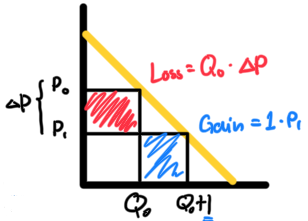
\includegraphics[width=0.4\columnwidth]{MR.png}
\end{wrapfigure}
\fbox{$MR = \frac{\Delta Rev(Q)}{\Delta Q} = P(Q) + Q \frac{\Delta P(Q)}{\Delta Q}$}
Decrease price results in: \textbf{\textcolor{Blue}{gain}} in Rev from Q increases + \textbf{\textcolor{Red}{loss}} in Revenue from P reduction for all units.
\Hint{If demand curve linear, MR has same intercept and twice the slope. $P(Q) = 100 - Q \rightarrow MR = 100 - 2 Q$}

\begin{wrapfigure}{r}{0.4\columnwidth}
    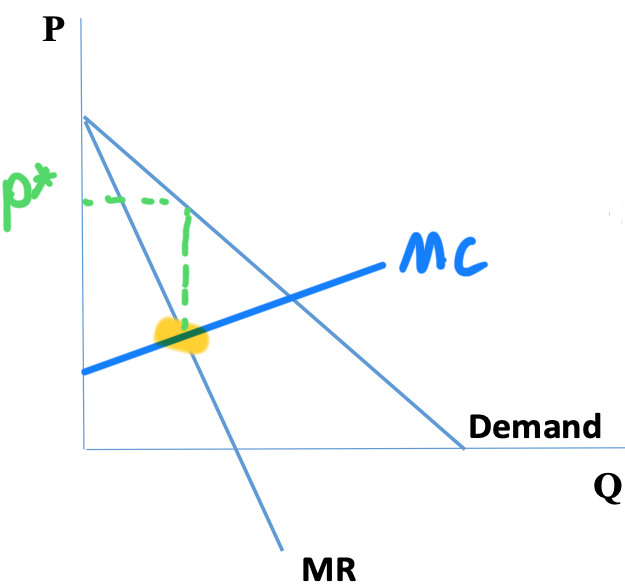
\includegraphics[width=0.4\columnwidth]{ProfitMax.png}
\end{wrapfigure}
\Green{Profix Maximization} optimal $Q^*$ when $MC(Q^*) = MR(Q^*)$. Then solve for optimal price $P^* =P(Q^*)$

\Green{Mark-up Formula} resulting from profit-max, $P^*$ satisfies: $\frac{P-MC}{P} = -\frac{1}{\epsilon}$ ($\epsilon$ is the demand elasticity).
Relatively more elastic markets (markets with more price-sensitive consumers) will face smaller markups (i.e., lower prices if costs are the same across markets).

\end{multicols}
\end{document}